\documentclass[a4paper]{article}
\usepackage{graphicx} 

%Russian-specific packages
%--------------------------------------
\usepackage[T2A]{fontenc}
\usepackage[utf8]{inputenc}
\usepackage[russian]{babel}
%--------------------------------------
\usepackage{afterpage}
\usepackage{xcolor}
\usepackage{hyperref}
\hypersetup{
    colorlinks,
    citecolor=black,
    filecolor=black,
    linkcolor=black,
    urlcolor=black
}
\usepackage{amsmath}
\usepackage{multicol}

\numberwithin{equation}{section}

\title{{\Huge Грустная аналитическая геометрия}}
\author{МКН-116}
\date{1 семестр}

\begin{document}
\begin{titlepage}
    \maketitle
    \pagecolor{yellow}\afterpage{\nopagecolor}
    \vfill
    \begin{center}
        
\includegraphics[width=\textwidth]{103-1032417_transparent-anime-girl-sad.png}
    \end{center}
    \vfill
    \vfill
\end{titlepage}

\tableofcontents

\newpage

\section{Векторная алгебра}

% \subsection{Деление отрезка в заданном отношении}
\paragraph{Деление отрезка в заданном отношении.} 
Найдем координаты точки M на отрезке AB, которая делит этот отрезок в отношениии $\frac{\lambda}{\mu}$.

\begin{equation}
x = \frac{\mu x_1 + \lambda x_2}{\lambda + \mu}, \:
y = \frac{\mu y_1 + \lambda x_2}{\lambda + \mu}, \:
z = \frac{\mu z_1 + \lambda z_2}{\lambda + \mu}
\end{equation}
\paragraph{Преобразование координат из полярных в декартовы.}
Полярная система определена, если задана точка $O$ (полюс), исходящий из полюса луч $l$ (полярная ось).
Положение точки $M$ фиксируется двумя числами: радиус-вектором $r=|\vec{OM}|$ и углом $\phi$ (полярным углом) между полярной осью и вектором $\vec{OM}$.
\begin{multicols}{2}
    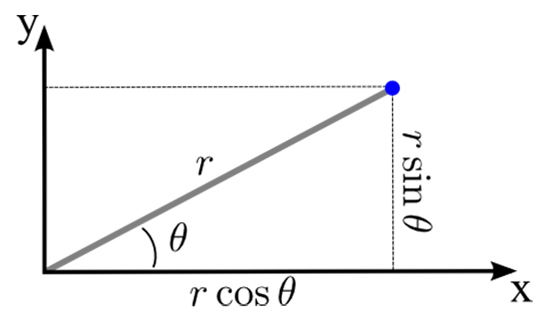
\includegraphics[width=0.4\textwidth]{Polar-Cartesian-Coordinates-Feature.jpg}
    \columnbreak
    \null \vfill 
    \begin{gather*}
        x = r cos\phi \\
        y = r sin\phi \\
        r = \sqrt{x^2 + y^2}
    \end{gather*}
    \vfill \null
\end{multicols}
\paragraph{Замена базиса}
Положение новго базиса относительно старого должно быть задано: 
\begin{gather*}
    e'_1 = \alpha^1_1 e_1 +\alpha^2_1 e_2 + \alpha^2_1 e_3 \\ 
    e'_2 = \alpha^1_2 e_1 +\alpha^2_2 e_2 + \alpha^2_2 e_3 \\ 
    e'_3 = \alpha^1_3 e_1 +\alpha^2_3 e_2 + \alpha^2_3 e_3 
\end{gather*}
Матрицей перехода называется матрица, в столбцах коротой стоят компоненты векторов $e'_1, e'_2,e'_3$ в старом базисе.
\begin{gather*}
    \Sigma = 
    \begin{pmatrix}
        \alpha^1_1 & \alpha^1_2 & \alpha^1_3\\
        \alpha^2_1 & \alpha^2_2 & \alpha^3_2\\
        \alpha^3_1 & \alpha^3_2 & \alpha^3_3
    \end{pmatrix}
\end{gather*}
Координаты вектора в старом и новом базисе связаны уравнением
\begin{gather*}
    X' = \Sigma^{-1} X \\ 
    \begin{pmatrix}
        x'  \\
        y'  \\
        z'  \\
    \end{pmatrix} = \Sigma^{-1} \cdot
    \begin{pmatrix}
        x  \\
        y  \\
        z  \\
    \end{pmatrix}
\end{gather*}
Обратную матрицу можно найти по методу Гаусса или с помощью формулы
\begin{gather*}
    \Sigma^{-1} = \frac{1}{\det \Sigma}\cdot \Sigma^V, \quad 
    \begin{pmatrix}
        A_{11} & A_{21} & A_{31} \\
        A_{12} & A_{22} & A_{32} \\
        A_{13} & A_{23} & A_{33} \\
    \end{pmatrix},
\end{gather*}
где $A_{ij}$ - алгебраическое дополнение к элементам матрицы $\Sigma$.
\paragraph{Изменение системы координат.}

\newpage

\section{Исследование уравнения второго порядка}
В общей декартовой системе координат линия второго порядка может быть задана уравнением:
\begin{equation}
    \begin{gathered}
        Ax^2 + 2Bxy + Cy^2 + 2Dx + 2Ey + F = 0, \\
        A^2 + B^2 + C^2 \neq 0
    \end{gathered}
\end{equation}

Избавимся от слагаемого, содержащего $xy$.
Для этого введем новую декартову прямоугольную систему координат, у которой старые координаты выражаются через новые следующим образом:
\begin{equation}
    \begin{cases}  x = x' cos \phi - y' sin \phi \\ y = x' sin \phi + y' cos \phi \end{cases}
\end{equation}

В новых координатаз уравнение примет вид:
\begin{equation}
    \begin{gathered}
        A(x\cos \phi - y' sin \phi)^2 + 2B(x\cos \phi - y' sin \phi)(x\sin \phi + y' cos \phi) + \\ + C(x\sin \phi + y' cos \phi)^2 + ... = 0
    \end{gathered}
\end{equation}
Все что отмечено многоточием нас сейчас не интересует.
Раскроем скобки и получим, что в новой системе координат коэффициент при $x'y'$ равен:
$ B' = -Asin \phi cos \phi + B(cos^2 \phi - sin^2 \phi) + Csin \phi cos \phi $

\end{document}